\subsection{Benchmark}

The authors provided us with three graphs in order to test our
different implementations of the Tutte method.\\

These graphs have the following characteristics :

\begin{center}
\begin{tabular}{|c|c|c|}
\hline
Graph & number of vertices & number of edges \\
\hline
aiir\_traffic & 14693 & 63403\\
imdb & 9488 & 33942\\
migration & 14318 & 49460\\
\hline
\end{tabular}
\end{center}


The histogram (figure \ref{histo}) shows the different times of execution
that we obtain through our different implementations:

\begin{figure}[!h]
  \centering
  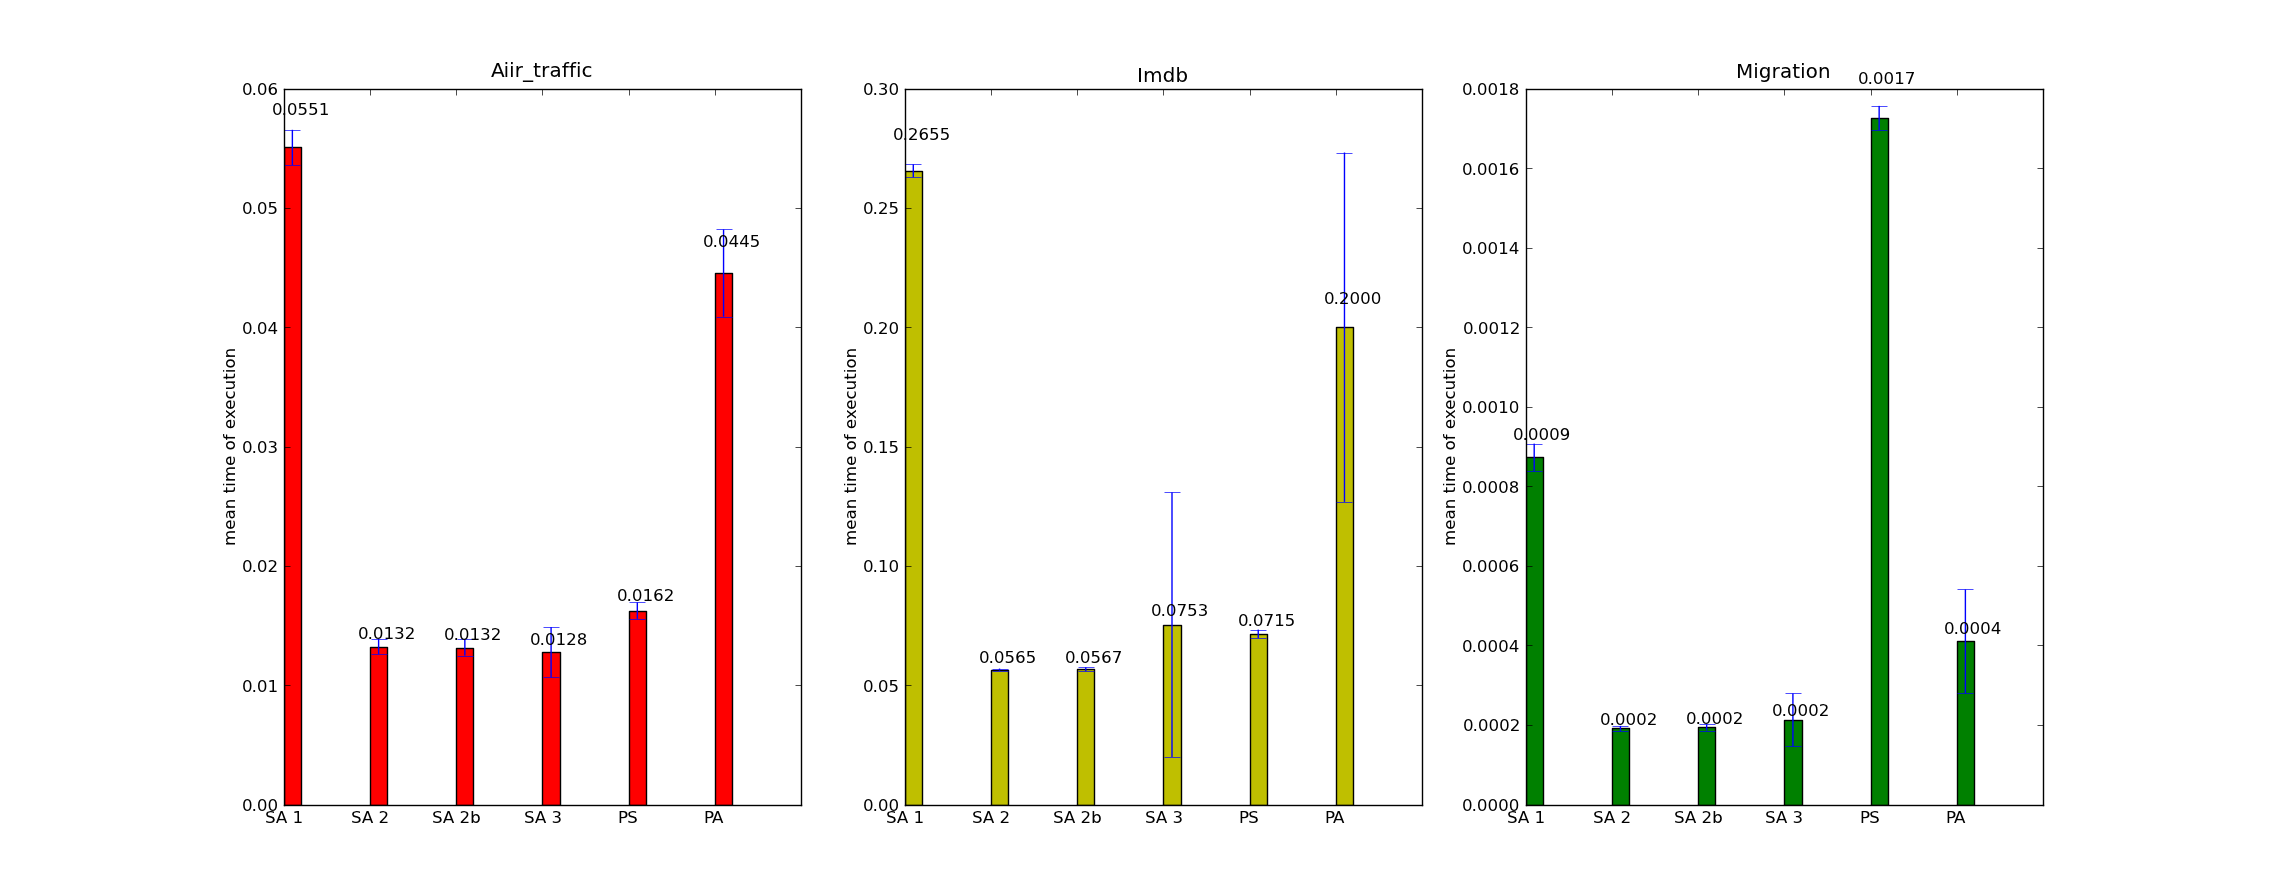
\includegraphics[scale=0.4]{img/histogramme.png}
  \caption{All the mean times of execution}
  \label{histo}
\end{figure}

\underline{\bf Definition of each tags above a bar}
\begin{dinglist}{70}
\item [SA 1]: Tutte sequential asynchronous version on the first data structure;
\item [SA 2]: Tutte sequential asynchronous version on the second data structure;
\item [SA 2b]: Tutte sequential asynchronous version on the second data structure with usage of Vec2f;
\item [SA 3]: Tutte sequential asynchronous version on the third data structure;
\item [PS]: Tutte parallel synchronous version on the second data structure;
\item [PA]: Tutte parallel asynchronous version on the first data structure;
\end{dinglist}

The mean times of computation showed on the figure \ref{histo} are been
obtained over 1000 executions of each algorithm. The configuration of the
computer that has done the executions is :
\begin{description}
\item {Processor}: Intel Core i5-2410M
\item {RAM} : DDRIII 6 GB
\end{description}

One can notice that the best implement is the sequential asynchronous
version on the second data structure. Also, the parallel implementations
are not the faster one certainly because the number data to treat is not
enough great.

\subsection{Not planar graph}
The results we get here are not as good as we expected. Although the
computation time is quite improved, the produced graphs are not planar. The
reason is that the provided graph has some fixed nodes inside the
grid. Consequently, after the call of our implementation of the Tutte
Algorithm, some edges crossing (due to those fixed nodes) appear and remove
the planar property of the graph.

As an explanation, we can say that moving nodes tend to be oriented to the 
side which has the highest level of fixed nodes.(see the figure \ref{mauvais_1}). 
With such a graph, a mobile node which is opposite to the side with numerous
edges will move to this side and create an edge-crossing (see the figure \ref{mauvais_2}).

\begin{figure}[!h]
  \begin{minipage}[!h]{.5\linewidth}
   \centering
   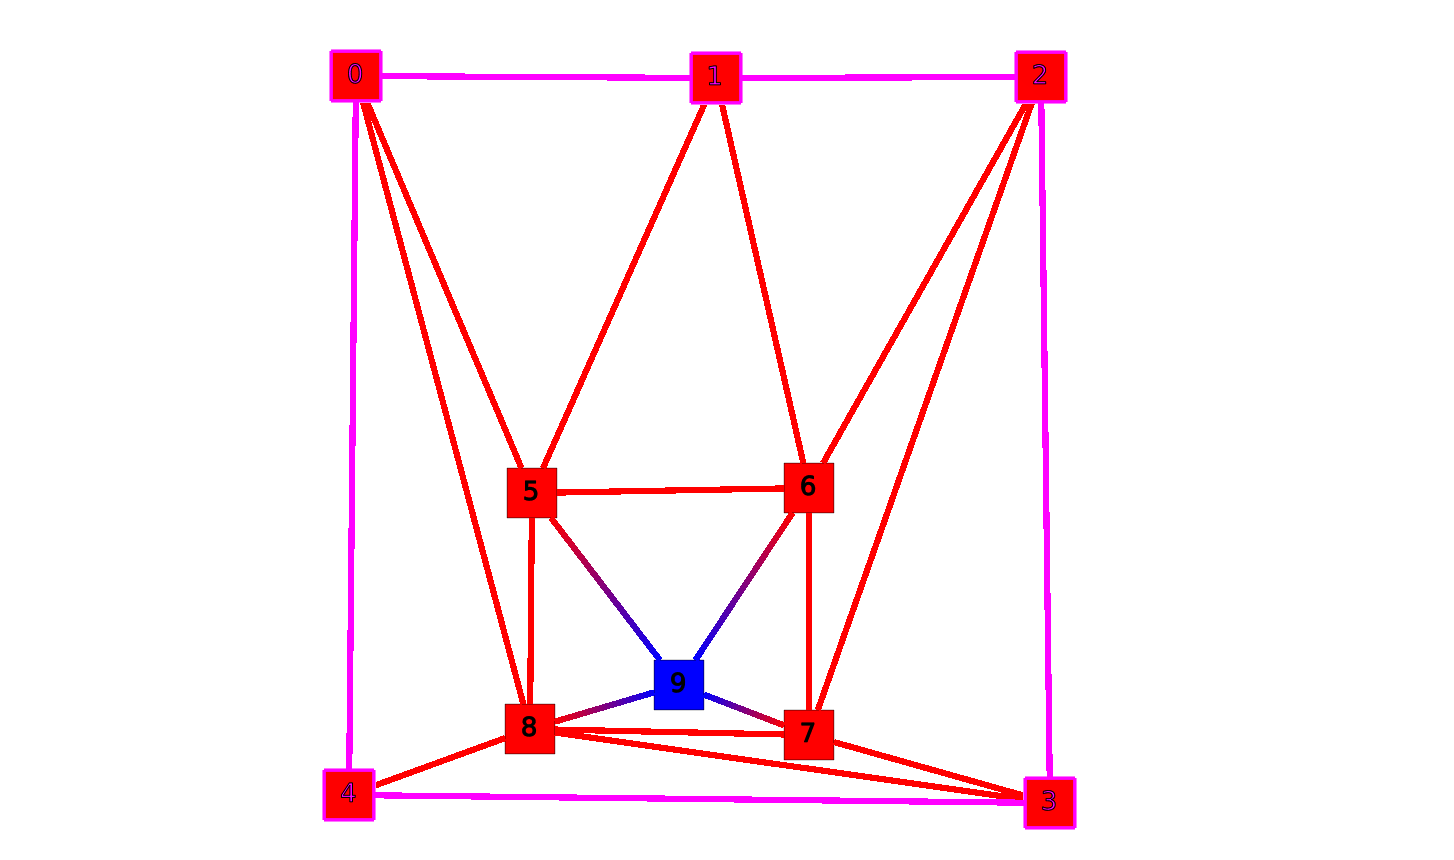
\includegraphics[scale=0.27]{snapshots/constate_fix_init.png}
   \caption{The initial graph. The blue node is fixed}
   \label{mauvais_1}
 \end{minipage} \hfill
 \begin{minipage}[!h]{.45\linewidth}
   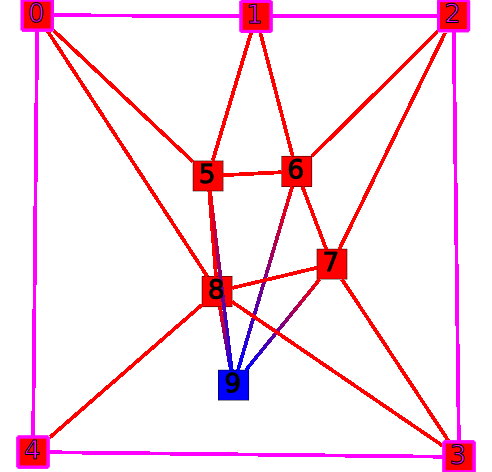
\includegraphics[scale=0.45]{snapshots/constate_probleme.png}
   \caption{The set not correctly modified}
   \label{mauvais_2}
 \end{minipage}
\end{figure}

%\newpage 

You can notice that if all the nodes in the interior of boundaries are mobile, then the graph produced stay planar (see figure \ref{correct_1} and \ref{correct_2}).

\begin{figure}[!h]
  \begin{minipage}[!h]{.5\linewidth}
    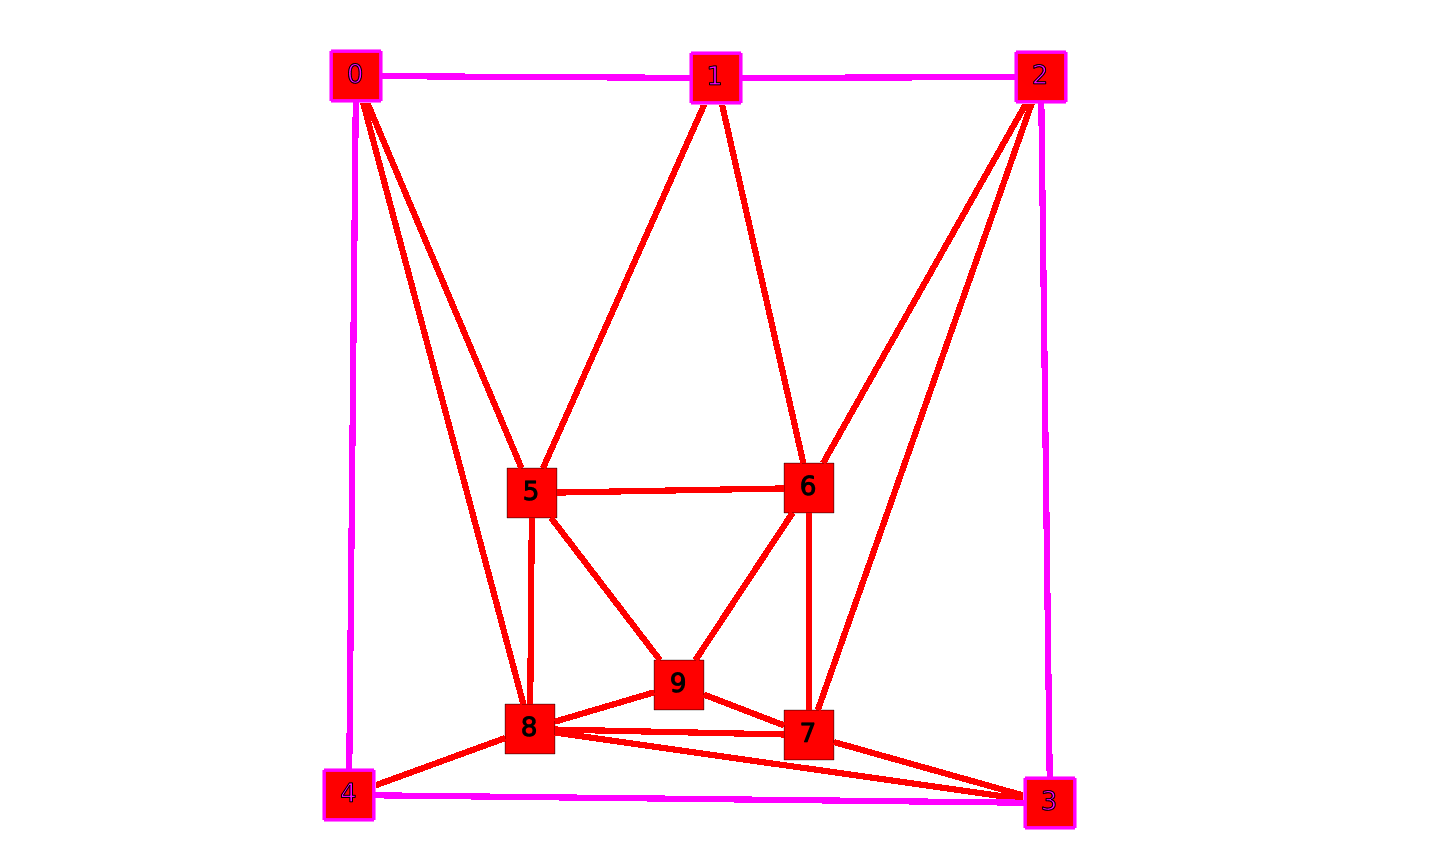
\includegraphics[scale=0.27]{snapshots/constate_mobil_init.png}
    \caption{The initial graph with all interior nodes mobile}
    \label{correct_1}
  \end{minipage}
  \begin{minipage}[!h]{.55\linewidth}
    \centering
    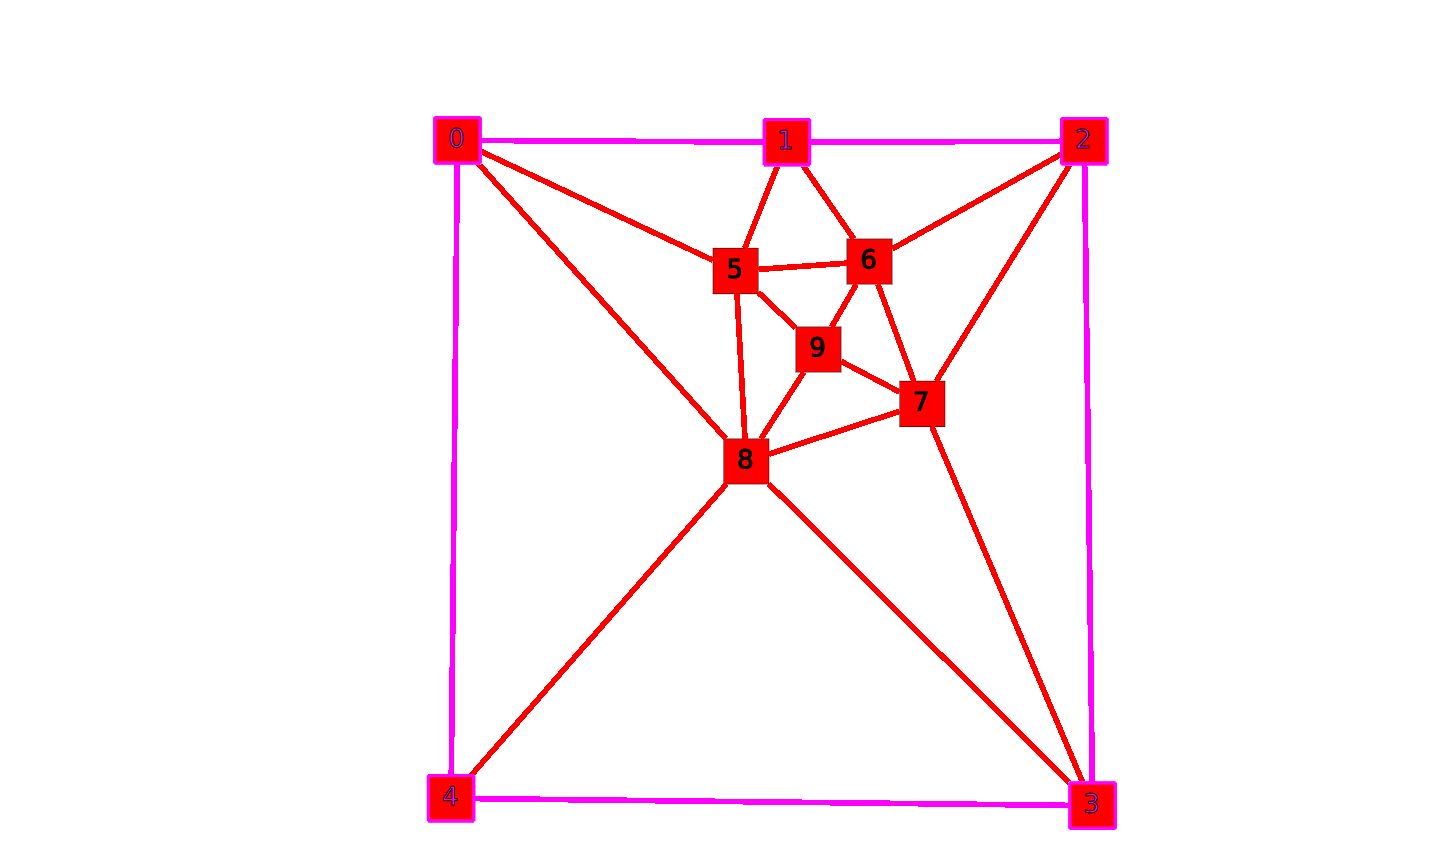
\includegraphics[scale=0.29]{snapshots/constate_nikel.png}
    \caption{The graph correctly modified}
    \label{correct_2}
  \end{minipage} \hfill
\end{figure}
